\documentclass{beamer}
\usecolortheme[RGB={0,102,51}]{structure}
\usetheme[height=9mm]{Rochester}
\usepackage{animate}

\usepackage{amsfonts,amssymb,amscd,amsmath,mathrsfs,amsthm}

\usepackage{tikz}
\usetikzlibrary{lindenmayersystems}
\pgfdeclarelindenmayersystem{A}{%
  \symbol{F}{\pgflsystemstep=0.6\pgflsystemstep\pgflsystemdrawforward}
  \rule{A->F[+A][-A]}
}
\usepackage{minted}
\usepackage{caption}
\usepackage{subcaption}


% Usetheme:
%
%\usetheme{Helsinki}

\author{Steven Glasford}
\title{Modeling a Fungal Competition on a Plant.}
\date{\today}
%\thanks{Dr. Ivan Yegorov}




\begin{document}

% Frame 1
\begin{frame}
\maketitle
\end{frame}
%todo: add background photo from https://bygl.osu.edu/sites/default/files/field/image/tar%20spot%20punctatum%203%20%20S%20Fair%208-20-16.jpg to the title page it has a good photo of fungal pathagen

\AtBeginSection[]  % A frame titled `Content' is added before every new section starts.
{
\begin{frame}<beamer>
\frametitle{Content} % Title of the automatically added frame
\tableofcontents[currentsection]   % List all the structure components that call this frame (section, subsection, subsubsection,...; add `current')
\end{frame}
}


% Section `Introduction'; sections are defined outside of frames. They may lead to the automatic inclusion of additional frames, see above.
\section{What is a pathogen?}
% \subsection{Motivation}
\begin{frame}{Pathogens are costly.}
    Pathogens make living things sick. \newline
    
    COVID-19 is a significant pathogen. \newline
    
    Pathogens can end up costing gigantically. \newline
    
    2016 alone saw \$540 billion in agricultural damages from plant pathogens. 
    
        
    \begin{center}
    \includegraphics[ height = 4cm ]{money.jpg}
    \end{center}
\end{frame}

\begin{frame}{What is fungal competition?}
    We will be looking at parasitic pathogenic fungi, such as leaf rust. 
    When you can see the rust it is in the spore producing phase.\newline
    
    Limited resources, fighting for resources, not each other.\newline
    
    The host has finite resources and fungus does not want to kill plant (loses all of its food).
    
    \begin{center}
        \includegraphics[ width = 7cm, height = 4.6cm ]{Figure_poplar_leaf_rust.pdf}
    \end{center}
\end{frame}

\begin{frame}{Closer inspection of Fungi}
    The pathogens we will be investigating exploit leaf tissue. \newline

    % Mycelia expand into the current leaf. 
    Latency period as fungus makes investment in mycelial growth.  \newline

    % Spore production gets to more leaves.

    \begin{center}
        \includegraphics[ width = 9.5cm, height = 5cm ]{Figure_biotrophic_pathogens.pdf}
    \end{center}
\end{frame}

\section{Modeling}
% \subsection{Description}
\begin{frame}{Description of fungal equations.}
    We focus on a single season, on a single plant, without evolution. \newline
    
    Unrealistic in the wild (wild is complicated), we can still get useful results, especially in laboratory conditions.

    \begin{center}
        \includegraphics[ width = 10.5cm, height = 6cm ]{Figure_scheme.pdf}
    \end{center}
\end{frame}

% \subsection{Assumptions}
\begin{frame}{Convert to equations}
    Using the information from the previous slide, we can get:
    
    $$ 
    \left\{ \begin{aligned}
    & \frac{d M_1(t)}{dt} \:\: = \:\: (1 - u_1(t)) \, f_1(M_1(t), M_2(t)) \: - \: g(M_1(t)), \\
    & \frac{d M_2(t)}{dt} \:\: = \:\: (1 - u_2(t)) \, f_2(M_1(t), M_2(t)) \: - \: g(M_2(t)), \\
    & f_i(M_1, M_2) \:\: \stackrel{\mathrm{def}}{=} \:\: \nu(n_1 M_1 \, + \, n_2 M_2) \: \rho(M_i), \quad i = 1,2, \\
    & 0 \leqslant u_i(t) \leqslant 1, \quad i = 1,2, \quad t \in I_T, \\
    & M_1(0) = M_1^0, \quad M_2(0) = M_2^0.
    \end{aligned} \right.
    $$
    \pause
    These are the resource allocation strategies.\newline
    
    \pause
    
    When $u = 0$ mycelial production, $u = 1$ spore production.
    A little of both when in between between 1 and 0.
\end{frame}

\begin{frame}{Assumptions}
    $n$ is the lesion density and is assumed to be constant for simplicity. \newline\pause
    
    $$
    f(M) \: \stackrel{\mathrm{def}}{=} \: \nu(n M) \, \rho(M),
    $$
    is the nutrient flux. \newline
    
    $\rho(M)$ is amount of resources flowing through a single mycelium.
    
    $ \nu(n M) $ describes the negative influence of competing mycelia. \newline\pause
    
    We assume the resident is cohort 1, and the mutant is cohort 2.
\end{frame}

% \subsection{Equations}
\begin{frame}{Uninvadable strategies}
    The cohorts are not fighting each other. They are fighting for limited resources. \newline\pause
    
    The competition forms a zero-sum feedback game: the resident defends, the mutant is offensive. \newline\pause
    
    We assume that the cohorts use an uninvadable strategy. Each cohort tries its best and tries to ensure the other cohort does not fully invade. \newline\pause
    
    An uninvadable strategy is also known as an evolutionary stable strategy.
\end{frame}


% \subsection{Method of solving.}
\begin{frame}{Uninvadable equations}
    Let $ J_i $ be the marginal fitness (the amount of success of cohort $i$)
    $$J_i(u_1, u_2) = \: \int\limits_{I_T} u_i(t) f_i(M_1(t), M_2(t)) \, \delta \, e^{-\mu t} \, dt \: $$ of cohort~$ i $. \newline\pause
    
    We can then say that the resident is not invaded if: $$ \: J(u_1, u_2) \: \stackrel{\mathrm{def}}{=} \: J_2(u_1, u_2) - J_1(u_1, u_2) \: \leqslant \: 0. $$ \pause
    
    We are most interested in modeling when $J$ forms a saddle point (i.e., $J = 0$).\newline
    
    Further derivation and analysis of $J$ can be found in \cite{YegorovGrognardMailleretHalkettBernhard2019}
    
\end{frame}

\begin{frame}{Differential Game}
    The previous slides give us the following:
    $$
    \begin{aligned}
    & J(u_1(\cdot), u_2(\cdot)) \:\: = \:\: J_2(u_1(\cdot), u_2(\cdot)) \: - \: J_1(u_1(\cdot), u_2(\cdot)) \:\: = \\
    & = \:\: \int\limits_{I_T} (u_2(t) \, f_2(M_1(t), M_2(t)) \: - \: u_1(t) \, f_1(M_1(t), M_2(t))) \: \delta \, e^{-\mu t} \: dt \:\:
    % \longrightarrow \\
    \\& \longrightarrow \:\: \inf_{u_1(\cdot)} \: \sup_{u_2(\cdot)} \:\: \mbox{or} \:\:
    \sup_{u_2(\cdot)} \: \inf_{u_1(\cdot)} \, ,
    \end{aligned}
    $$ \pause
    this describes how the first cohort tries to maximize its resistance to the second, and vice versa.\newline
    
    $\inf$ is the infimum (lower bound) $\sup$ is the supremum (upper bound).\newline
    
    $\inf\sup=\sup\inf$ describes a saddle point (unstable equilibrium).
    
\end{frame}

\section{Execution and Code}
% \subsection{Code.}
\begin{frame}{Numerical Analysis}
    The equations we are working with are nonsmooth, and nonlinear making them difficult to solve exactly. Numerical analysis is essential \newline\pause

    We use computers to simulate this system. \newline\pause
    
    We can convert our equations into Hamilton--Jacobi--Isaacs equation (HJI). \newline\pause
    
    We can then solve the HJI with ROC-HJ (Reachability, Optimal Control, and Hamilton-Jacobi equations).
\end{frame}

\begin{frame}{Hamilton--Jacobi--Isaacs equation}
    For brevity, we exclude the reasoning behind converting to a Hamiltonian.\newline\pause
    
    \mathcal{H} is the Hamiltonian, describes the minimax/maximin (saddle point) of J.
    
    \begin{equation*}
    \resizebox{\hsize}{!}{
        \left\{ 
            \begin{aligned}
                & \frac{\partial V(t, M_1, M_2)}{\partial t} \: + \: \mathcal{H}
                \left( t, M_1, M_2, \frac{\partial V(t, M_1, M_2)}{\partial M_1},
                \frac{\partial V(t, M_1, M_2)}{\partial M_2} \right) \:\: = \:\: 0, \\
                & V(T, M_1, M_2) \: = \: 0, \\
                & t \in [0, T], \quad (M_1, M_2) \: \in \: G.
            \end{aligned} 
        \right.  
        \label{15}
    }
    \end{equation*}
\end{frame}

\begin{frame}{Resource Control Strategy}
    The Hamiltonian minimax (maximin) condition reduces to the following:
    \begin{equation*}\resizebox{\hsize}{!}{
        \begin{aligned}
            & u_1(t, M_1, M_2) \:\: = \:\: 
            \begin{cases}
                0, & e^{-\mu t} \: + \: \frac{\partial V(t, M_1, M_2)}{\partial M_1}
                 \: < \: 0, \\
                1, & e^{-\mu t} \: + \: \frac{\partial V(t, M_1, M_2)}{\partial M_1}
                \: > \: 0, \\
                \mbox{arbitrary from} \:\: [0, 1], & e^{-\mu t} \: + \: \frac{\partial
                V(t, M_1, M_2)}{\partial M_1} \: = \: 0,
            \end{cases} \\
            & u_2(t, M_1, M_2) \:\: = \:\: 
            \begin{cases}
                0, & e^{-\mu t} \: - \: \frac{\partial V(t, M_1, M_2)}{\partial M_2}
                \: < \: 0, \\
                1, & e^{-\mu t} \: - \: \frac{\partial V(t, M_1, M_2)}{\partial M_2}
                \: > \: 0, \\
                \mbox{arbitrary from} \:\: [0, 1], & e^{-\mu t} \: - \: \frac{\partial V(t,
                M_1, M_2)}{\partial M_2} \: = \: 0.
            \end{cases}
        \end{aligned}  
        \label{16}
    }\end{equation*}
    where $u_1$ corresponds to the resource allocation strategy for cohort 1 (resident), and $u_2$ fits cohort 2 (mutant).
\end{frame}

\begin{frame}{Reverse Time}
    ROC-HJ works backward (enables the user to start with an outcome and see how it started). \newline\pause
    
    We must rewrite our equations in reverse.
    
    \begin{equation*}\resizebox{\hsize}{!}{
        \left\{ 
            \begin{aligned}
                & \frac{\partial V(T - \tau, M_1, M_2)}{\partial \tau}    \:\: + \:\:
                \max_{u_1 \in [0, 1]} \: \min_{u_2 \in [0, 1]} \:
                \left( -H \left( T - \tau, \, M_1, \, M_2, \, u_1, \, \\
                & \qquad
                u_2, 
                % {}^{{}^{{}^{{}^{{}^{}}}}}
                \right. \right. 
                \left. \left. \frac{\partial V(T - \tau, M_1, M_2)}{\partial M_1}, \,
                \frac{\partial V(T - \tau, M_1, M_2)}{\partial M_2}     \right) \right) \:\: =
                \:\: 0, \\
                & V(T - \tau, M_1, M_2) \left|_{\tau = 0} \right. \: = \: 0, \\
                & \tau \in [0, T], \quad (M_1, M_2) \: \in \: G,
            \end{aligned} 
        \right.  \label{75}
    }\end{equation*}
\end{frame}

\begin{frame}{Example and Basic Parameters}
    We use the Finite Difference Method,\newline
    Second-order time discretization, \newline
    Find the saddle strategies.\newline
    
    ROC-HJ \cite{ROCHJ2019}.
    
    \begin{figure}[ht]
        \inputminted[
            frame=lines,
            framesep=2mm,
            baselinestretch=1.2,
            fontsize=\footnotesize,
            firstline=15, 
            lastline=17]{c}{code/data.h}
        \caption{Configurations of descriptive variables}
        \label{code:defaults}
    \end{figure}
\end{frame}


% \subsection{Output}
\begin{frame}{Output}
    ROC-HJ produces a large amount of data in .dat files.\pause
    \begin{figure}[ht]
        \inputminted[
            frame=lines,
            framesep=2mm,
            baselinestretch=1.2,
            fontsize=\footnotesize,
            firstline=1, 
            lastline=5]{c}{code/VF20_100.dat}
        \caption{The first five lines from when $\tau=20$ produced from ROC-HJ.}
        \label{code:datfile}
    \end{figure}
    describes a point on a plane (x,y) and the direction of the vector.\newline
    It needs to be graphed to produce meaningful results.
\end{frame}

\section{Graphs and Analysis}

\begin{frame}{Graphs 1/4}
    % $t=48.825$ is a sort of inflection point.
    
    \begin{center}
        \includegraphics[ height = .37\textwidth]{Figure_5c_1.pdf}
        \includegraphics[ height = .37\textwidth]{Figure_5c_2.pdf}
    \end{center}
    
\end{frame}

\begin{frame}{Graphs 2/4}
    \begin{center}
        \includegraphics[ width = 4cm, height = 2.3cm ]{Figure_5a_1.pdf}
        \includegraphics[ width = 4cm, height = 2.3cm ]{Figure_5a_2.pdf} \\
        \includegraphics[ width = 4cm, height = 2.3cm ]{Figure_5b_1.pdf}
        \includegraphics[ width = 4cm, height = 2.3cm ]{Figure_5b_2.pdf} \\
        \includegraphics[ width = 4cm, height = 2.3cm ]{Figure_5c_1.pdf}
        \includegraphics[ width = 4cm, height = 2.3cm ]{Figure_5c_2.pdf}
    \end{center}

White is mycelial growth, gray is spore production.

\end{frame}

\begin{frame}{Graphs 3/4}
    \begin{figure}
        \centering
        \begin{subfigure}{.48 \textwidth}
            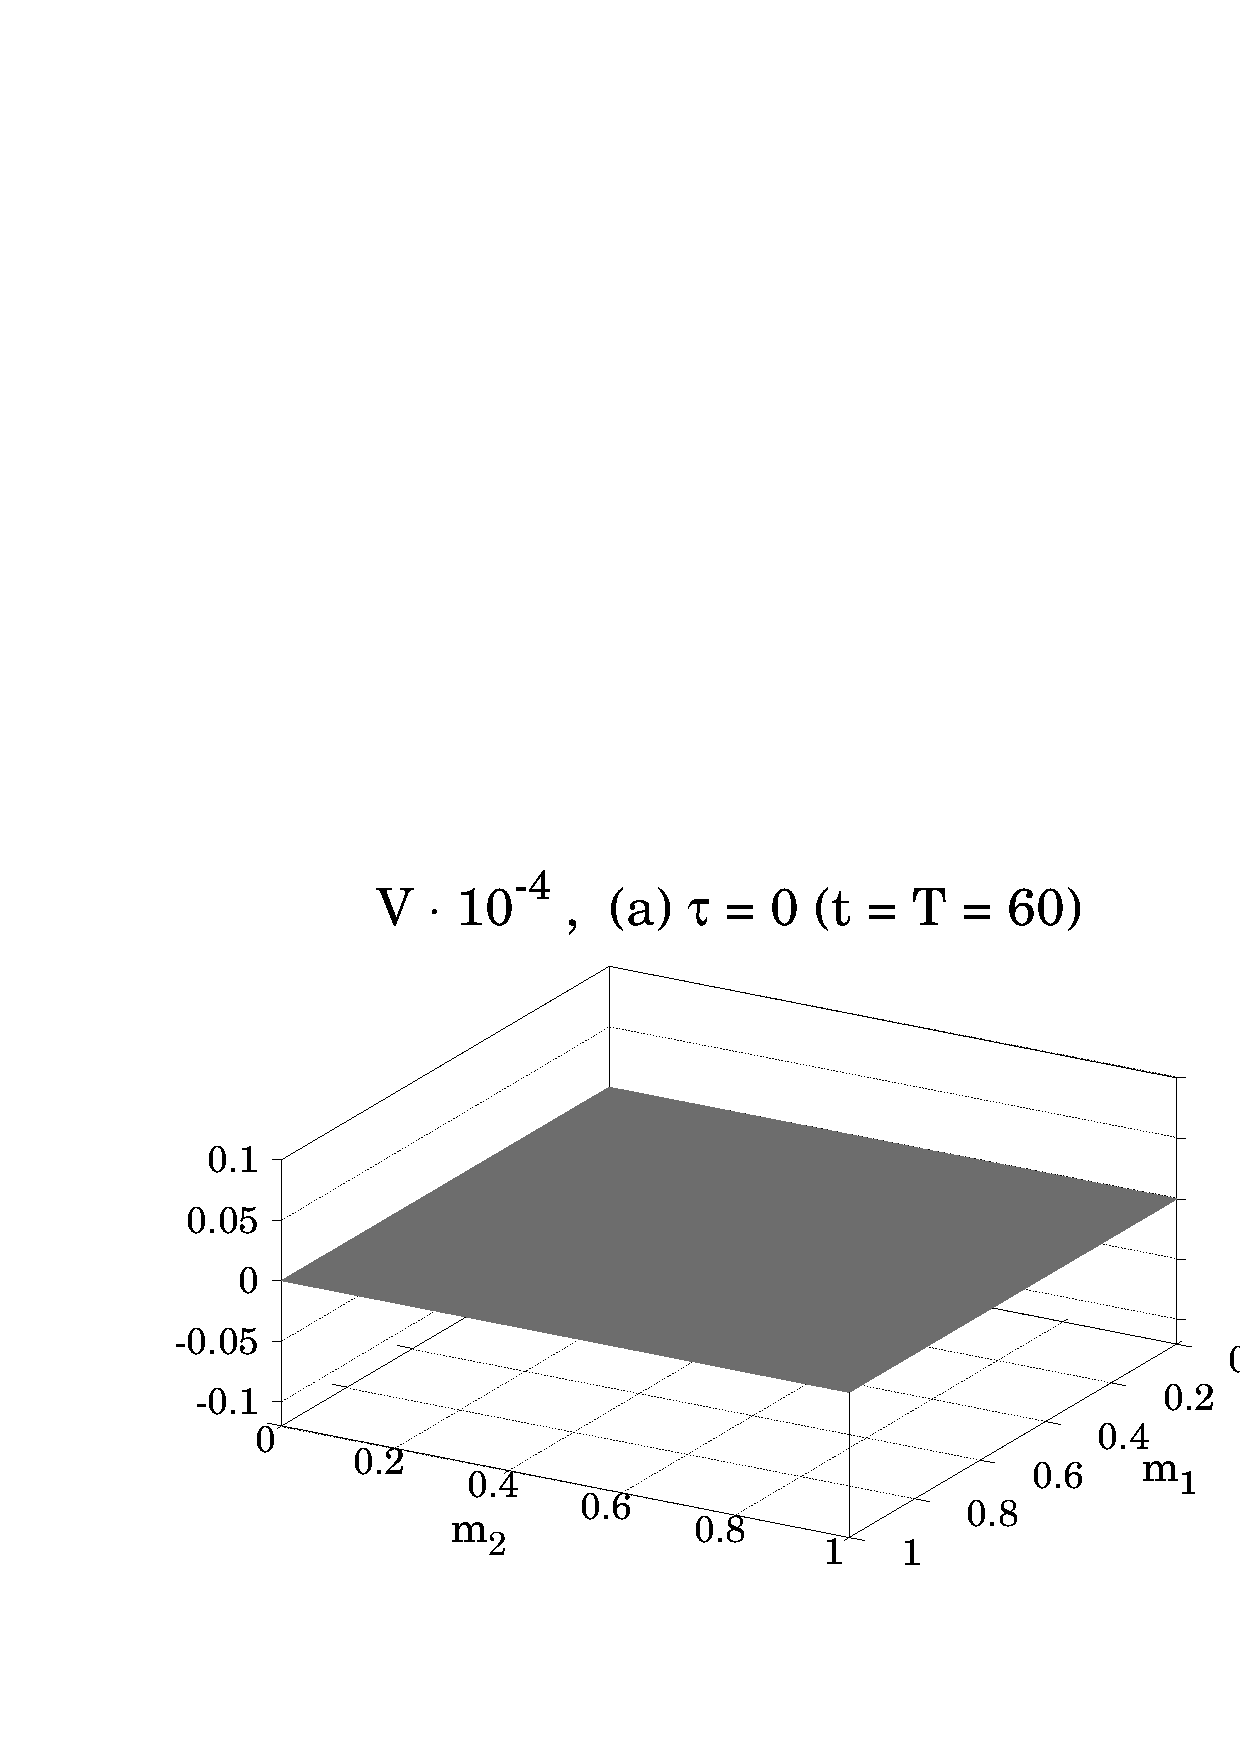
\includegraphics[width = \textwidth]{figures/Figure_4a.pdf}
            \label{fig_4_a}
        \end{subfigure}
        \begin{subfigure}{.48 \textwidth}
            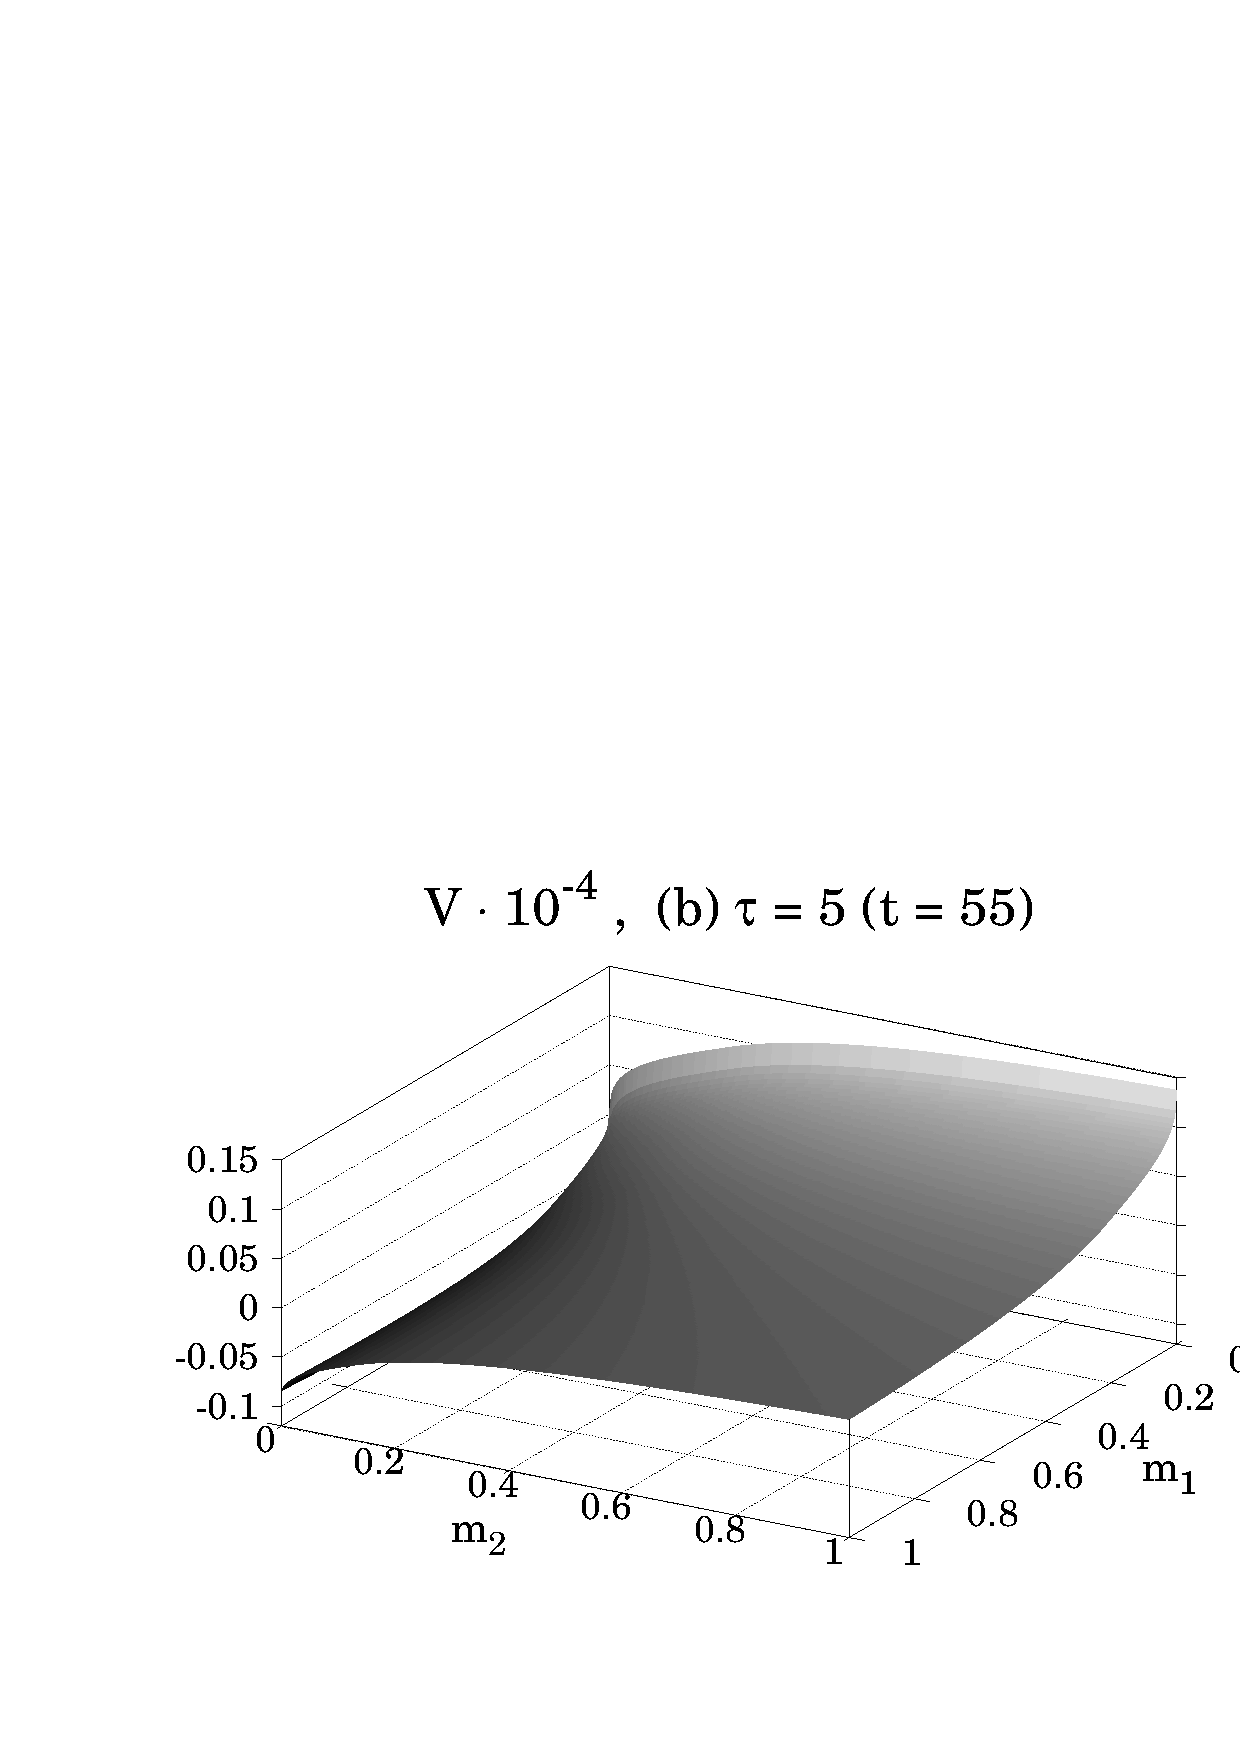
\includegraphics[width = \textwidth]{figures/Figure_4b_1.pdf}
            \label{fig_4_b}
        \end{subfigure}
        \begin{subfigure}{.48 \textwidth}
            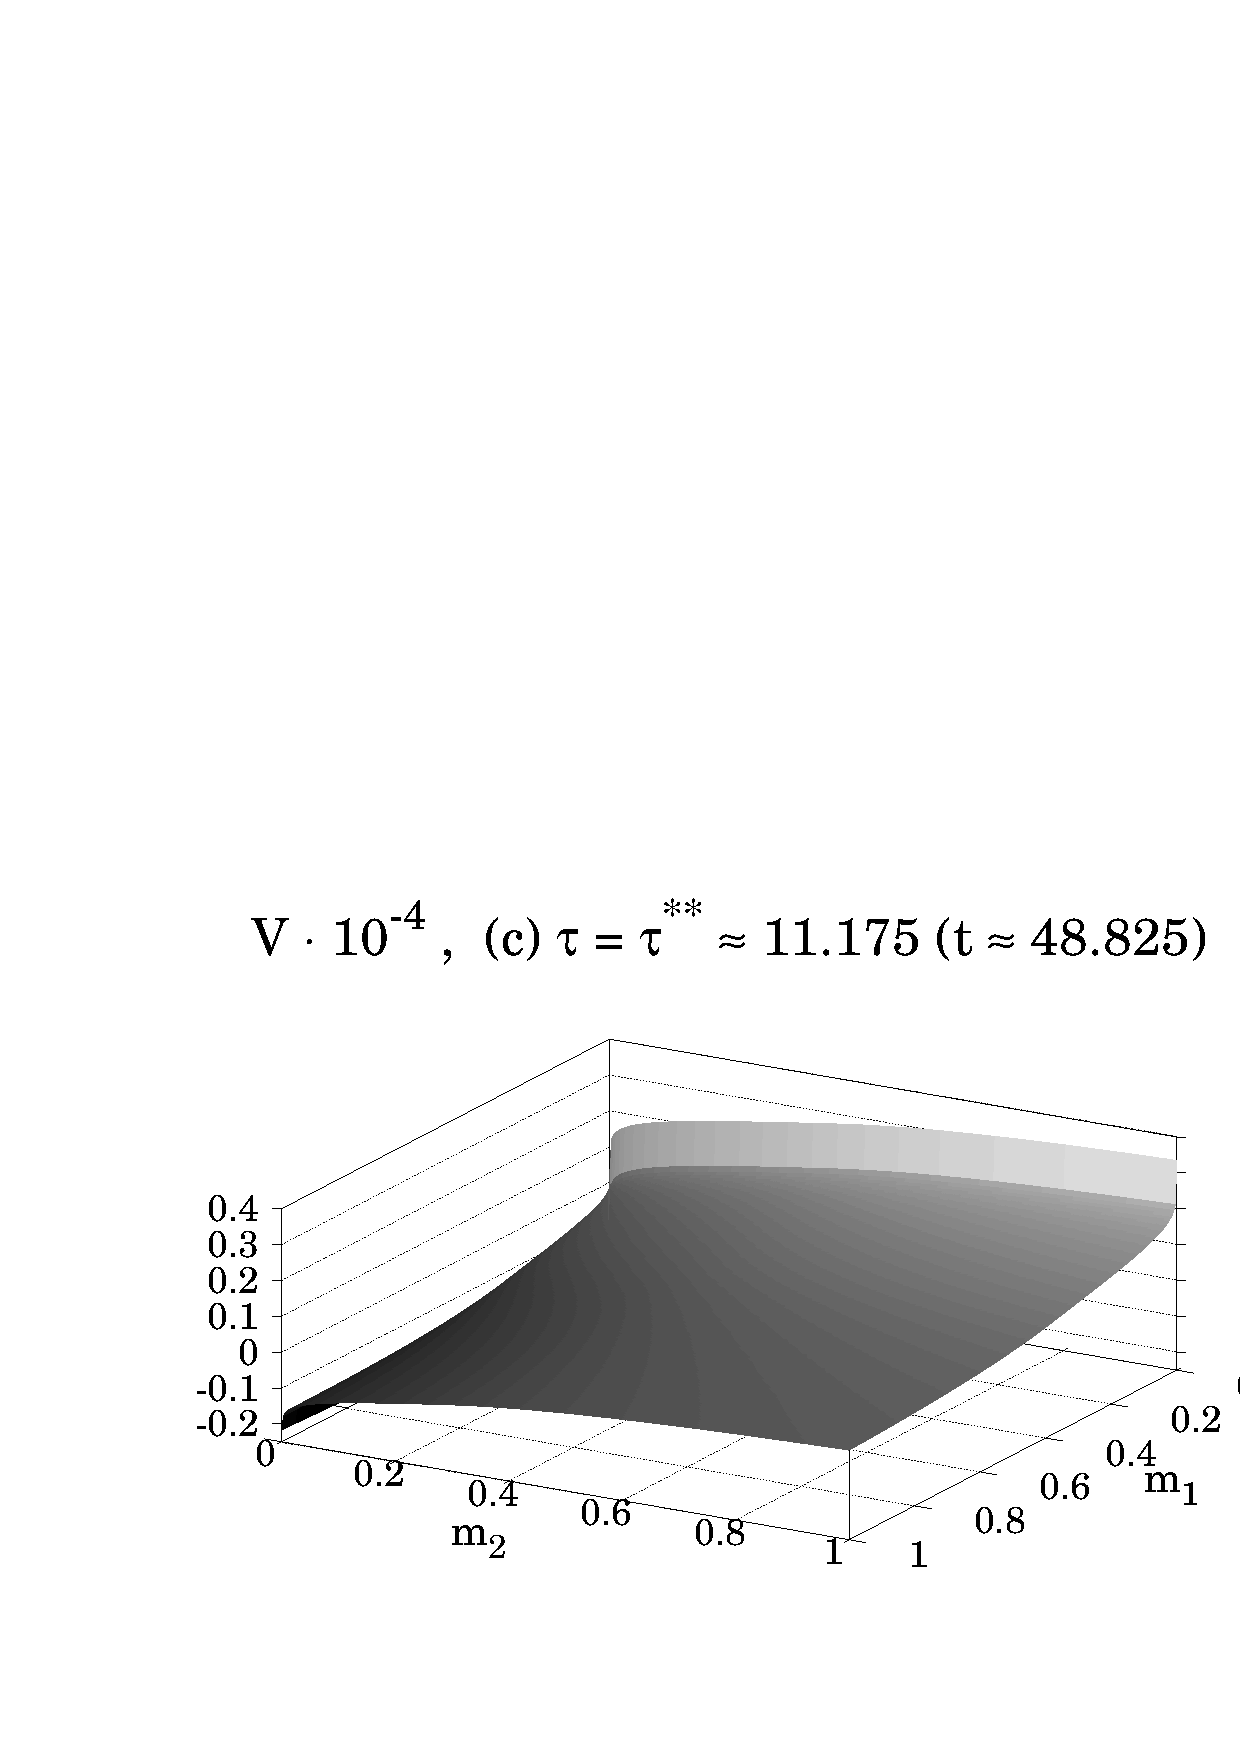
\includegraphics[width = \textwidth]{figures/Figure_4c_1.pdf}
            \label{fig_4_c}
        \end{subfigure}
        \begin{subfigure}{.48 \textwidth}
            \includegraphics[width = \textwidth]{figures/Figure_4d_1.pdf}
            \label{fig_4_d}
        \end{subfigure}
    \label{Fig_4}
    \end{figure}
\end{frame}

\begin{frame}{Graphs 4/4}
    \begin{figure}
        \center{ 
            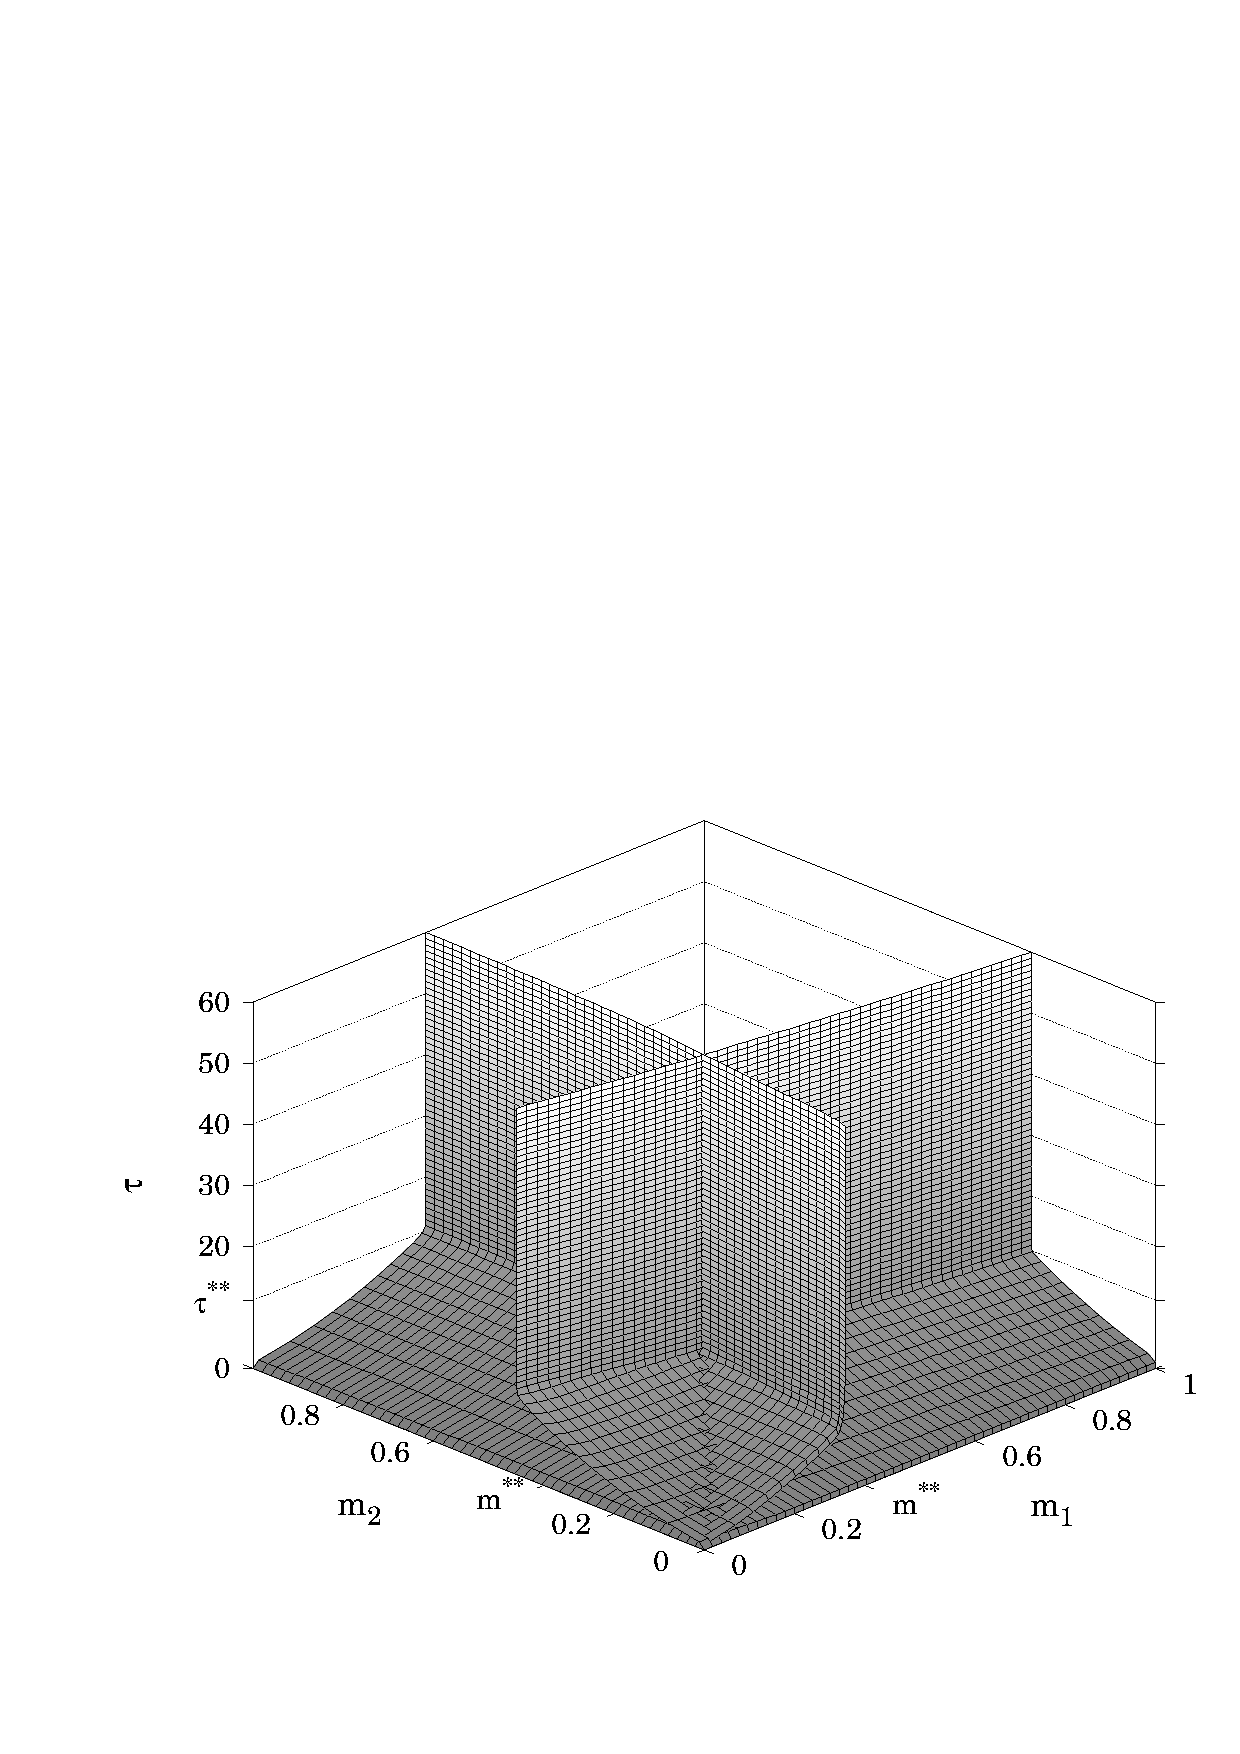
\includegraphics[width = 0.98 \textwidth]{figures/Figure_7.pdf} 
        }
        \bf \caption{\it The four control turnpike switching surfaces in the three-dimensional space~$ (m_1, m_2, \tau) $. A turnpike is the most efficient route in order to reach the steady-state equilibrium.}
        \label{Fig_7}
    \end{figure}
\end{frame}



\section{Conclusion}
% \subsection{Analysis, and Limitations}
\begin{frame}{Model Limitations}
    \begin{itemize}
        \item Our model is not super general.\pause
        \item One-seasonal\pause
        \item No evolution (plant or fungal)\pause
        \item Single plant\pause
        \item Ignores plant diversity \pause
        \item Ignores plant regrowth and other tolerances\pause
        \item Ignores actual fighting between fungi (some fungi produce toxins to kill opponents)\pause
    \end{itemize}
    
    \vspace{.4cm}More research is needed to investigate more dynamic systems.\newline
    
    Still very useful, sets a benchmark to test against in future analysis.
\end{frame}


\begin{frame}{End statements}
    Future analysis will include previously stated factors.\newline\pause
    
    We looked at strategies for nearly equivalent fungi competing with each other, fighting for resources. \newline
    
    Thank you, Dr. Ivan Yegorov!
    
\end{frame}

\begin{frame}{References}
    \bibliographystyle{plain}
    \bibliography{steven_sources.bib}
\end{frame}

\end{document}